The Module manager is useful for creating a modular view of large networks, i.e.
a more compact network,  without loosing any details of the initial global
network. To achieve this goal, we are using the ``nested networks`` feature of Cytoscape, introduced with the version 2.7.

\subsection{Create Network of Modules}
\textbf{Plugins$\Rightarrow$BiNoM 2.1$\Rightarrow$BiNoM Module Manager$\Rightarrow$Create Network of Modules}\\
This function creates a new network from a list of subnetworks (subnetworks are selected in the network list located on the left panel of the Cytoscape application, see figure~\ref{Create_network_of_modules}).\\
In the new network that is created, each node represents a module, pointing in fact to a subnetwork. 

\includegraphics[width=20pt,height=20pt]{graphics/warning} Module names, node names and network names must be different.\\\\

In order to visualize a subnetwork contained in a module, select the node
corresponding to the module, then right-click with the mouse and choose ''Nested
Network$\Rightarrow$Go to Nested Network`` from the contextual menu.

\begin{figure}
\centering
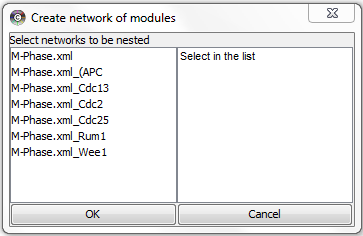
\includegraphics[width=0.8\textwidth]{graphics/Create_network_of_modules}
\caption{Dialog for selecting the networks that will be included in a module.}
\label{Create_network_of_modules}
\end{figure}

\subsection{Create Connections between Modules}
\textbf{Plugins$\Rightarrow$BiNoM 2.1$\Rightarrow$BiNoM Module Manager$\Rightarrow$Create Connections between Modules}\\
This function creates edges linking modules from all the edges of the selected network.\\
The links are simplified, no distinction is made between left and right (molecule flow), there is no duplication if two interactions are the same.\\
A warning message is displayed if there are duplicated or absent nodes.

\begin{figure}
\centering
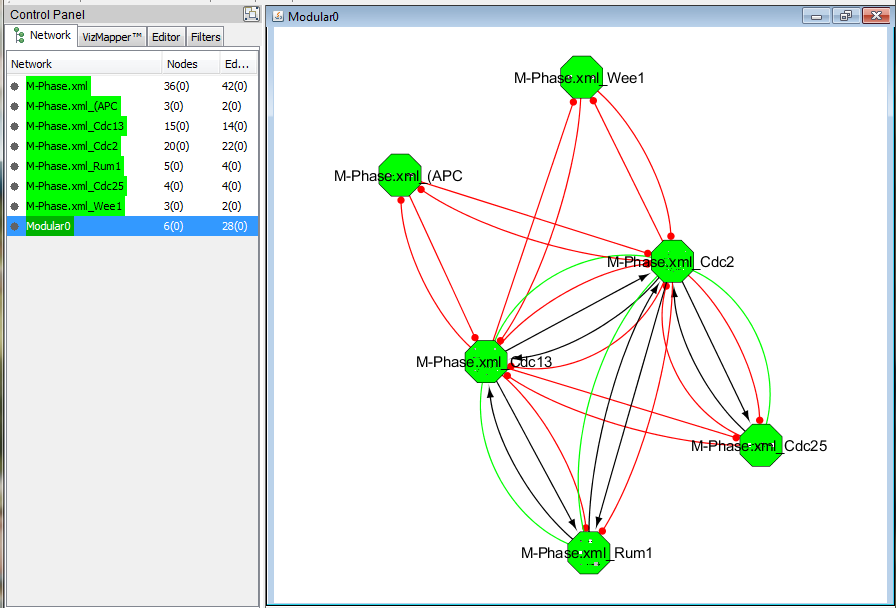
\includegraphics[width=0.8\textwidth]{graphics/M-Phase_Material_Modular}
\caption{To generate this figure, the M-Phase network is divided into
subnetworks by using the ''get material component'' function. The modular view
is created by selecting different subnetworks and applying the function ``create a network of modules``. Then, to create the links between the modules, the function "Create
connections between modules" links modules according to the reference global network. The function "Find common nodes in modules" creates intersection edges.}
\label{M-Phase_Material_Modular}
\end{figure}

\subsection{Create Modules from Networks}
\textbf{Plugins$\Rightarrow$BiNoM 2.1$\Rightarrow$BiNoM Module Manager$\Rightarrow$Create Modules from Networks}\\
This function creates modules in the active network from a list of sub-networks (sub-networks are selected in the network list)\\
All edges are kept. See edge attribute PREVIOUS\_ID for their origin.\\
The attribute BIOPAX\_NODE\_TYPE is set to “pathway” (see visual style BiNoM BioPAX).\\
\includegraphics[width=20pt,height=20pt]{graphics/warning} All nodes of sub-networks must be found once in the active network (no intersection between sub-networks).

\subsection{Agglomerate the Nearest Nodes in Modules}
\textbf{Plugins$\Rightarrow$BiNoM 2.1$\Rightarrow$BiNoM Module Manager$\Rightarrow$Agglomerate the Nearest Nodes in Modules}\\
This function creates modules and a modular view by agglomerating the nearest nodes in the active network (see the algorithm description in section~\ref{Agglomeration_by_shortest_path}.\\\\
There are two input parameters in order to limit the computational time and the number of modules:
\begin{itemize}
\item Maximal distance between nodes or modules in number of edges,
\item Maximal number of nodes in modules.
\end{itemize}
Confirm creation if agree with displayed result (see dialog~\ref{Agglomerate_in_modules_dialog}).\\\\
Sub-networks are created and gathered in a packed network as the function "Create modules from networks" (see figure~\ref{M-Phase_packed}).
\begin{figure}
\centering
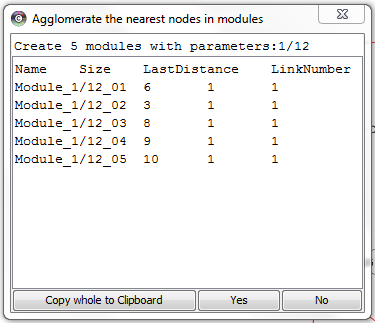
\includegraphics[width=0.8\textwidth]{graphics/Agglomerate_in_modules_dialog}
\caption{This window displays modules, number of node, last distance and number of links of agglomerating process. Yes lauches the process of agglomerating.}
\label{Agglomerate_in_modules_dialog}
\end{figure}
\begin{figure}
\centering
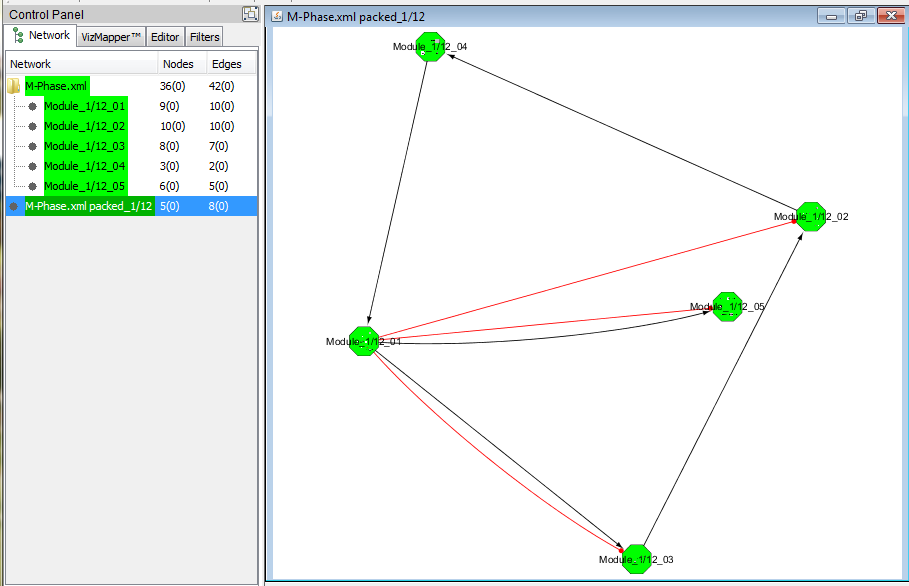
\includegraphics[width=0.8\textwidth]{graphics/M-Phase_packed}
\caption{M-Phase is got by creating network from modules, modules created by agglomerating the nearest nodes (maximal distance=1, maximal size=12 nodes).}
\label{M-Phase_packed}
\end{figure}

\subsection{List Nodes of Modules and Network}
\textbf{Plugins$\Rightarrow$BiNoM 2.1$\Rightarrow$BiNoM Module Manager$\Rightarrow$List Nodes of Modules and Network}\\
This function list the nodes of the global network and nodes included in modules.\\
The results in the text box can be simply copied in a spreadsheet through the clipboard.

\subsection{Find Common Nodes in Modules}
\textbf{Plugins$\Rightarrow$BiNoM 2.1$\Rightarrow$BiNoM Module Manager$\Rightarrow$Find Common Nodes in Modules}\\
Display in a text box the matrix of nodes (modules in columns, nodes in
rows, size of modules in last row, frequency in modules in last column). The result
is more easily usable after copying it in a spreadsheet.
(see~\ref{Common_nodes_in_modules}.\\\\
Create intersection edges with number of common nodes as attribute
(COMMON\_NODES), green edges in figure~\ref{M-Phase_Material_Modular}.\\\\
Create a node attribute containing the node numbers of modules (NODE\_NUMBER).\\\\
The Module Visual Style can be adapted to the wished visual aspect by hand in
the Cytoscape VizMapper, for example:

\begin{itemize}
\item To visualize NODE\_NUMBER: double click Node Size, select NODE\_NUMBER, continuous mapping, adjust width by graphical view.
\item To visualize COMMON\_NODES double click Edge Line Width, select COMMON\_NODES, continuous mapping, adjust width by graphical view.
\end{itemize}
\begin{figure}
\centering
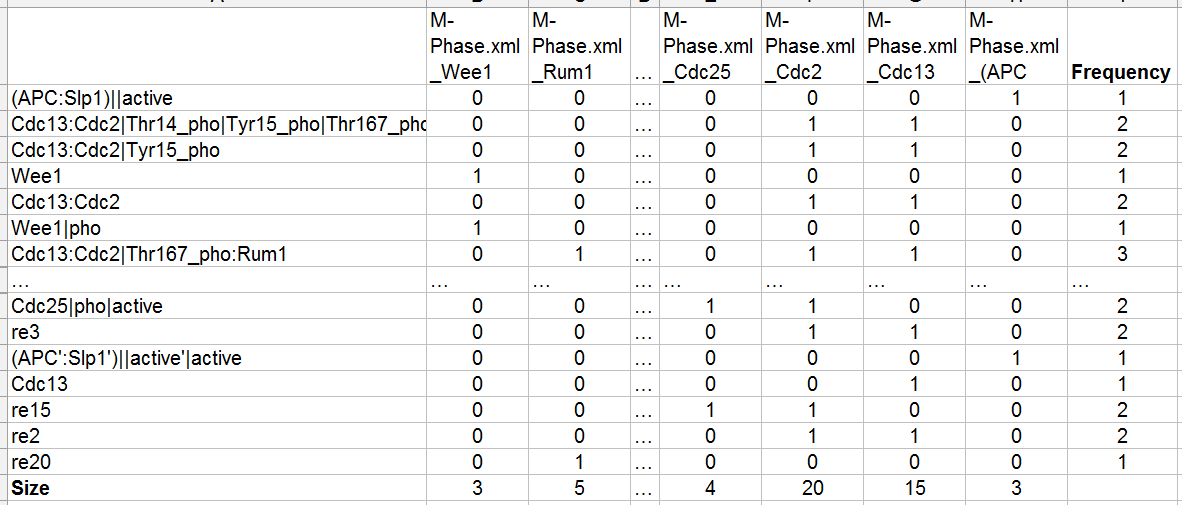
\includegraphics[width=0.8\textwidth]{graphics/Common_nodes_in_modules}
\caption{Matrix of nodes: modules in columns, nodes in rows, size of modules in last row, frequency in modules in last column.}
\label{Common_nodes_in_modules}
\end{figure}

\subsection{Assign Module Names to Node Attribute}
\textbf{Plugins$\Rightarrow$BiNoM 2.1$\Rightarrow$BiNoM Module Manager$\Rightarrow$Assign Module Names to Node Attribute}\\
Function to create a node attribute (named as the modular network), containing module names. This attribute may be used to visualize modules in the reference network.

\subsection{List Components of Species in Network and Modules}
\textbf{Plugins$\Rightarrow$BiNoM 2.1$\Rightarrow$BiNoM Module Manager$\Rightarrow$List Components of Species in Network and Modules}\\
Function to list the different components of a given species (their names must respect BiNoM syntax). This can be useful to name modules.

\subsection{Create Network from Union of Selected Modules}
\textbf{Plugins$\Rightarrow$BiNoM 2.1$\Rightarrow$BiNoM Module Manager$\Rightarrow$Create Network from Union of Selected Modules}\\
Function to create a network from the union of selected modules and its corresponding module in the current network (named by module names separated by \&).

\subsection{Create Network from Intersection of 2 Selected Modules}
\textbf{Plugins$\Rightarrow$BiNoM 2.1$\Rightarrow$BiNoM Module Manager$\Rightarrow$Create Network from Intersection of 2 Selected Modules}\\
Function to create a network from the intersection of 2 selected modules and its corresponding module (named by module names separated by \textbar.\\\\
The user must confirm for deleting the common nodes in the selected modules.

\subsection{Recreate Lost Connections inside Modules}
\textbf{Plugins$\Rightarrow$BiNoM 2.1$\Rightarrow$BiNoM Module Manager$\Rightarrow$Recreate Lost Connections Inside Modules}\\
Function to recreate the connections inside modules which may have been lost by modularizing operations.

\subsection{Destroy Networks Unused as Module}
\textbf{Plugins$\Rightarrow$BiNoM 2.1$\Rightarrow$BiNoM module manager$\Rightarrow$Destroy Networks Unused as Module}\\
Select networks to be deleted among a list of networks which are not used as modules in the current network (simplify cleaning session).
